\documentclass{beamer}
\usepackage{beamerthemesplit}

%\usepackage{pgfpages}
%\pgfpagesuselayout{resize to}[a4paper,landscape,border shrink=5mm]
%\pgfpagesuselayout{2 on 1}[a4paper,portrait,border shrink=5mm]
%\pgfpagesuselayout{8 on 1}[a4paper,portrait,border shrink=5mm]

\usepackage{ngerman}
\usepackage[applemac]{inputenc}
\usepackage{colortbl}
\usepackage{hyperref} 
\usepackage{graphicx}

\date{\today}
\author{markus.degen@fhnw.ch}
\institute{FHNW}
\logo{
\includegraphics[height=0.4cm]{../fhnw.png}}
\title {Netzwerke und Datenkommunikation}

\newcommand{\orangecell}{{\cellcolor[rgb]{0.98,0.83,0}}}
\newcommand{\greencell}{{\cellcolor[rgb]{0.4,0.9,0.3}}}
\newcommand{\graycell}{{\cellcolor[gray]{0.8}}}
\newcommand{\olivecell}{{\cellcolor[rgb]{0.6,0.8,0.2}}}
\newcommand{\steelcell}{{\cellcolor[rgb]{0.7,0.8,0.9}}}
\newcommand{\linksymbol}{\tiny{$\hookrightarrow$}}
\newcommand{\myurl}[1]{{\color{violet}{\tiny{\url{#1}}}}}

\renewcommand{\figurename}{Fig}

\usetheme[secheader]{Boadilla}
%\setbeamercolor*{palette primary}{use=structure,fg=black,bg=green!5!white}
%\setbeamercolor*{palette secondary}{use=structure,fg=black,bg=green!15!white}
%\setbeamercolor*{palette tertiary}{use=structure,fg=black,bg=green!25!white}
%\setbeamercolor*{palette quaternary}{fg=white,fg=red}

\setbeamercolor*{palette primary}{use=structure,fg=black,bg=green!25!yellow!35!white!70}
\setbeamercolor*{palette secondary}{use=structure,fg=black,bg=green!35!yellow!45!white!70}
\setbeamercolor*{palette tertiary}{use=structure,fg=black,bg=green!45!yellow!65!white!70}
\setbeamercolor*{palette quaternary}{fg=white,fg=red}


\begin{document} % ===============================================================

%\frame{
%\tableofcontents 
%}



\section{ND01: ISO/OSI Modell L1-L2}
\subsection{\"Ubersicht}
\frame {
\frametitle{Unterrichtsbl�cke} %------------------------------------------
\small
\begin{tabular}{|p{0.02\textwidth}|p{0.7\textwidth}|p{0.18\textwidth}|}
\hline
{\cellcolor[gray]{0.8}} Bl & {\cellcolor[gray]{0.8}} Inhalt  & {\cellcolor[gray]{0.8}} Buch \\ \hline
 01 &  Einleitung, \"Ubersicht, Grundbegriffe  & \tiny{}\\ \hline
 
\orangecell 01 &\orangecell OSI-Modell: L1 und L2 &\orangecell \tiny{GS: 570-573} \\ \hline
\end{tabular}
}

%% LABOR 
%Knoppix reaktivieren
%Knoppix reaktivieren / Blockparit�t
%Routing / XML
%IP-Adressen
%ARP / Ethereal
%DHCP / Ethereal
%DNS
%HTML / HTTP
%Python
%Python
%Apache
%Apache
%W-Lan

\frame {
  \frametitle{Reale Kommunikationsstrecken}
  \hbox{\includegraphics[width=6cm]{rc.pdf}\includegraphics[width=4cm]{lowpass.pdf}}
}

\frame { %------------------------------------------
\frametitle{ND02: ISO/OSI Modell} 
\textbf{Lernziele f\"ur ND02}
\begin{itemize}
\item Layer 1: Sie kennen die wichtigsten \"Ubertragungsarten von digitalen Signalen \"uber
  analoge Kan\"ale und deren (physikalische) Limiten
\item �Layer 2: sie kennen die Aufgabe des Layer-2
\item Layer 2: 
\end{itemize}
}


\frame { %------------------------------------------
\frametitle{Serielle Daten�bertragung}
Wenn Daten von einem Rechner zu einem anderen �ber eine serielle Leitung (z.B. 2 Dr�hte) �bertragen werden
sollen, muss folgendes beachtet werden:
\begin{itemize}
\item Die Daten�bertragung muss Bit f�r Bit geschehen
\item Es muss eine Methode gefunden werden, der Gegenstelle 
	mitzuteilen, wann die �bertragung beginnt, bzw. endet (Daf�r
	gibt es verschiedene Methoden: Steuerzeichen, Start/Stopp Bits)
\item Wenn m�glich soll eine �bertragungsfehlererkennung
	m�glich sein.
\item Es muss auf beiden Seiten Einigkeit betreffend der
	verwendeten Codierung herrschen.
\end{itemize}
Siehe dazu:
\myurl{http://www.netzmafia.de/skripten/modem/dfue1.html\#1.2.2}
% Rechner-Rechner, 1/0, synchron/asynchron 
}


\frame { %------------------------------------------
\frametitle{Analoge Daten\"ubertragung}
\begin{itemize}
\item
Bei den bisherigen Beispielen wurde davon ausgegangen, dass
die beiden Kommunikationsseiten direkt �ber eine Leitung verbunden
werden k�nnen und so \alert{Basisband�bertragung} m�glich ist.
\item Wenn die Verbindung �ber das �ffentliche Telefonnetz\footnote{oder Wireless, Cable-TV, etc} 
	hergestellt wird, dann ist eine Basisband�bertragung nicht 
	m�glich, weil keine direkte Leitung vom Sender zum 
	Empf�nger besteht, es k�nnen nur T�ne im Bereich 300 Hz
	bis 3 kHz �bertragen werden
\item [$\rightarrow$] Einsatz von Modems notwendig
\end{itemize}
Siehe dazu:
\myurl{http://www.netzmafia.de/skripten/modem/dfue1.html\#1.2.3}
und GS, Kap. 7.2
% Modems (Netzmafia/GS) 
% http://www.netzmafia.de/skripten/modem/dfue1.html#1.2.3
}

\frame { %------------------------------------------
\frametitle{Modulationsverfahren}
\small
\begin{description}
\item [Frequenzmodulation] Es werden zwei Frequenzen zur Darstellung einer ''0'' und einer ''1''
	verwendet. Die Amplitude ist konstant.
\item [Amplitudenmodulation] Die Amplitude wird ver\"andert, je nachdem ob eine ''1'' oder eine ''0''
	\"ubertragen wird. Die Frequenz ist konstant.
\item [Phasenmodulation] Sowohl die Frequenz wie auch die Amplitude sind konstant, ein  Phasensprung
	um z.B. 180 Grad kennzeichnet eine ''0'' oder eine ''1''. 
\item [Kombination] Die Verfahren k\"onnen auch kombiniert werden, so erh\"oht sich die 
	Durchsatzrate. In der Praxis werden z.B. in der Phasenmodulation mehr als ein Phasensprung
	eingesetzt, so k\"onnen jeweils mehrere Bit \"ubtertragen werden, z.B. 
	\texttt{''00'' : 0 Grad, ''01'' : 90 Grad, ''10'' : 270 Grad, ''11'' : 180 Grad}. Das selbe kann 
	auch mit der Amplitude bzw. mit den Frequenzen gemacht werden.
	 Bei einer \alert{vollduplex Verbindung}, verwenden die beiden
	Modems (Originate, Answer) dabei auf verschiedenen Frequenzen.
\end{description}
% Modems (Netzmafia/GS) 
Siehe dazu: \myurl{http://www.netzmafia.de/skripten/modem/dfue1.html\#1.2.6}
}

%\frame { %------------------------------------------
%\frametitle{Stecker und Kabel}
%http://www.netzmafia.de/skripten/netze/netz5.html
%}

\frame { %------------------------------------------
\frametitle{Netztopologien}
Die Knoten in Netzwerken k\"onnen auf verschiedene Arten 
verbunden werden:
\begin{description}
\item [Sternf\"ormig] Ein zentrales System, bei welchem s\"amtliche
	Verbindungen zusammenlaufen. Wenn das Zentrale System ausf\"allt,
	f\"allt das ganze Netz aus. 
\item [Bussystem] Alle Knoten sind an ein gemeinsames Medium
	angeschlossen. Die Daten passieren jeden Knoten, der Zugriff
	auf den Bus ist nicht synchronisiert.
\item [Ringf\"ormig] Jeder Knoten ist mit zwei Nachbarknoten 
	verbunden. Ein ''Token'' wird im Ring rumgereicht, nur derjenige
	Knoten der das Token hat, darf auf den Bus senden.
\item [Vermascht] Jeder Knoten ist mit einer Anzahl Nachbarknoten
	verbunden, es f\"uhren verschiedene Wege von einem Knoten zu
	einem anderen (Redundanz).
\end{description}
Siehe dazu: \myurl{http://www.netzmafia.de/skripten/netze/netz1.html}
}




\frame { %------------------------------------------
\frametitle{Multiplexing}
\begin{columns}
\begin{column}{3cm}
\begin{center}
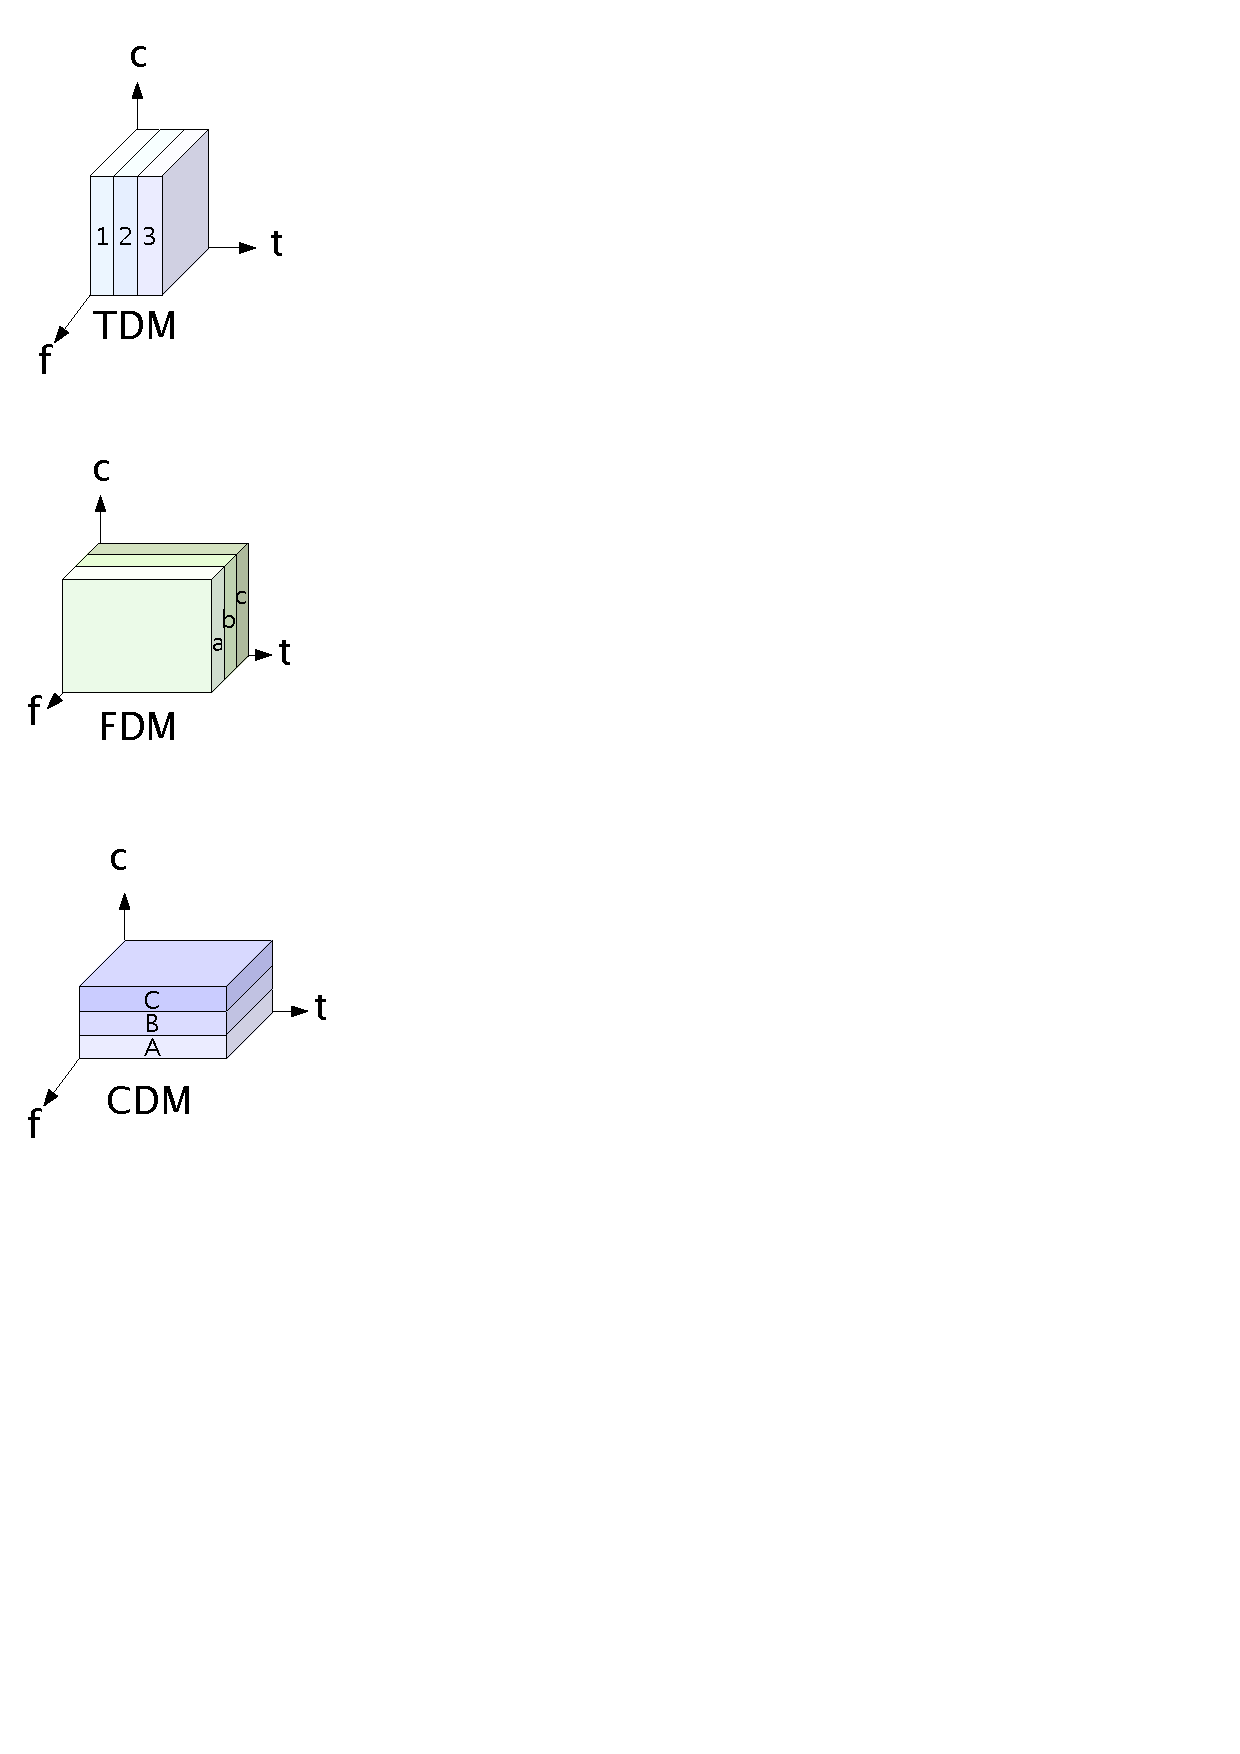
\includegraphics[width=0.7\textwidth]{multiplex.pdf}
\end{center}
\end{column}
\begin{column}{8cm}
\begin{itemize}
\item[TDM:] Time Division Multiplex: Die Kan\"ale werden zeitlich abwechselnd auf
	der selben Leitung \"ubertragen
\item[FDM:] Frequency Division Multiplex: Die Kan\"ale werden auf verschiedenen Frequenzen
	auf der selben Leitung \"ubertragen
\item[CDM:] Code Division Multiplex: Die Kan\"ale werden gleichzeitig mit verschiedenen
	Codes \"ubertragen
\end{itemize}
\end{column}
\end{columns}
}



\subsection{L2}
\frame { %------------------------------------------
\frametitle{Layer 2:  Data Link Layer}
\begin{columns}
\begin{column}{3cm}
\begin{center}
\includegraphics[width=0.7\textwidth]{osilayer2.pdf}
\end{center}
\end{column}
\begin{column}{8.8cm}
\small
\begin{itemize}
\item Der \emph{Data Link Layer} ist als \emph{Sicherungsschicht} verantwortlich
	f\"ur die Verbindung zwischen zwei Knoten
\item Die Bits von der Schicht 1 werden im Layer 2 zu \alert{Frames} zusammengefasst
	und mit Zusatzinformationen f\"ur die Fehlererkennung ausgestattet
\item Es erfolgt eine \emph{Flusssteuerung}, damit der Empf\"anger nicht 	
	mit Frames \"uberflutet wird 
\item Bei LAN's erfolgt eine weitere Unterteilung der Schicht 2:
\begin{itemize}
\item MAC: Media Access Control (Zugriff auf das \"Ubertragungsmedium)
\item LLC: Logical Link Control (Sicherung)
\end{itemize}
\end{itemize}
\end{column}
\end{columns}
}



\frame { %------------------------------------------
\frametitle{Fehlererkennende Codes}
\small
F\"ur die Erkennung von \"Ubertragungsfehlern (''Bitdreher''), werden verschiedene Methoden
eingesetzt, bei denen zus\"atzliche \alert{Redundanz} in die Daten eingef\"ugt wird. 
Fehlererkennung ist immer ein Tradeoff zwischen zus\"atzlicher Redundanz und Auftretenswahrscheinlichkeit des Fehlers.
\begin{description}
\item [Parit\"atsbits:] Pro Byte ein  z.B. zus\"atzliches Bit, welches die Anzahl der ''1'' 
	reflektiert (z.B. gerade Anzahl $\rightarrow$Parit\"atsbit=''0'').
\item [Pr\"ufsummen:] Auch CRC, Cyclic Redundancy Check. Es werden nach bestimmten
	Regeln Checksummen \"uber die Daten gebildet und mitgesendet, auf der Empfangsseite 
	wird die Pr\"ufsumme erneut gebildet und mit der mitgesendeten verglichen.
\item [Hammingcodes:] Die ''Unterschiedlichkeit'' der Codew\"orter wird ausgenutzt, damit
	Fehler erkannt und korrigiert werden k\"onnen. Wenn z.B. der Code nur die folgenden
	M\"oglichkeiten umfasst: 0000000000, 0000011111, 1111100000, 1111111111, 
	dann betr\"agt der ''Abstand'' zwischen den einzelnen Codew\"ortern $n$=5 Bit 
	(=Hammingdistanz) damit k\"onnen $n-1$ Bit Fehler erkannt werden.
\end{description}
}


\frame { %------------------------------------------
\frametitle{Beispiel f\"ur Parit\"atsbits}
\begin{center}
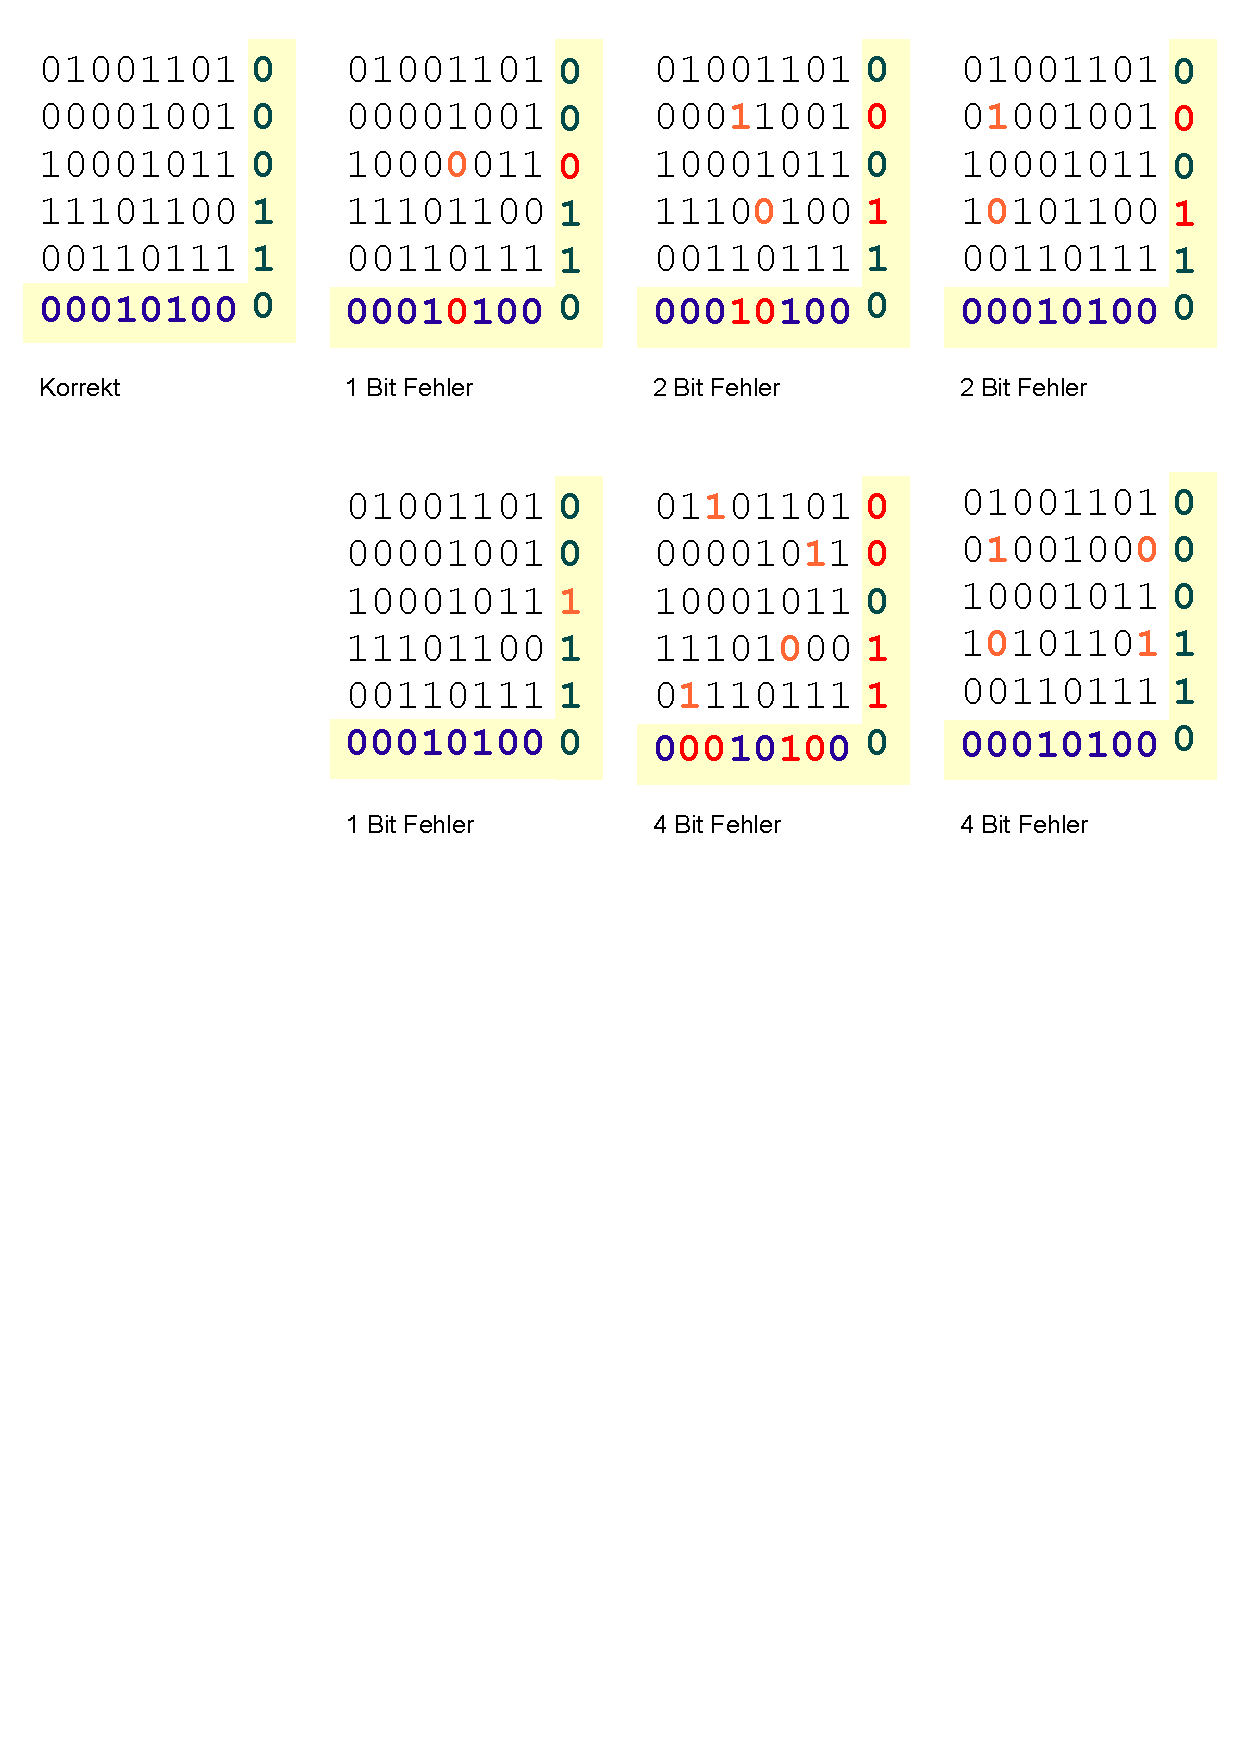
\includegraphics[width=0.8\textwidth]{blockparity.pdf}
\end{center}
}

\subsection{Abschluss}
\frame { %------------------------------------------
\frametitle{Abschluss} 
\textbf{Behandelte Themen:}
\begin{itemize}
\item Schichten 1 und 2 (Physical Layer, Data link Layer) vom ISO/OSI Modell
\end{itemize}
\textbf{M\"ogliche Pr\"ufungsfragen}
\begin{itemize}
\item Bezeichnen Sie alle Schichten des OSI-Modells. Welche Aufgaben
	haben die jeweiligen Schichten (L1 und L2) zu erf�llen  ?
\item Was genau wird unter Leitungsd�mpfung verstanden, vergleichen
	Sie die D�mpfungen in Kupfer- und Glasfaserleitungen. 
\end{itemize}
\textbf{Labor}
\begin{itemize}
\item \"Ubung zu Data Link Layer (Siehe Folgeseite)
\item Umgang mit Knoppix (Starten Sie Knoppix und versuchen 
	Sie herauszufinden, auf welche IP-Addresse (www.xxx.yyy.zzz)
	ihre Netzwerkkarte konfiguriert ist).
\end{itemize}
}


\frame { %------------------------------------------
\frametitle{\"Ubungen} 
\framesubtitle{Zu Data Link Layer}
\textbf{Blockparit\"at:}
\begin{itemize}
\item Codieren Sie ein Wort mit 5 Buchstaben mittels des ASCII-Codes
	in Bin\"arcode
\item Erg\"anzen Sie das Resultat mit \emph{gerader Blockparit\"at} (Wie Beispiel im Kurs)
\item F\"ugen Sie nun zwei korrigierbare ''1 Bit Fehler'' ein
\item Taschen Sie das Ergebnis mit einem Kollegen/einer Kollegin
\item Finden und korrigieren Sie die Fehler im erhaltenen Block
\item Decodieren Sie das Wort mittels ASCII-Tabelle
\item Vergleichen Sie das erhaltene Resultat
\end{itemize}
}



\end{document} 